\documentclass[uplatex,dvipdfmx,a4j,12pt]{jsarticle}

\usepackage[utf8]{inputenc}
\usepackage{graphicx}
\usepackage{amsmath}
\usepackage{comment}
\usepackage{listings,jvlisting} 
\usepackage{color}
\usepackage{url}
\usepackage{siunitx}
\usepackage[version=4]{mhchem}
\usepackage{paralist}
\usepackage{longtable}
\usepackage{multirow}
\usepackage[dvipdfmx]{hyperref}
\usepackage{pxjahyper}
\usepackage{enumitem}
\setlist[description]{parsep=5pt}
\setlist[enumerate]{parsep=5pt}
\usepackage{here}
\usepackage{mathtools}
\usepackage{amssymb}
\usepackage{physics}
\usepackage{mathcomp}
\usepackage{makecell}
\usepackage{subcaption}
\usepackage{tcolorbox}

\usepackage{cleveref}
\crefname{figure}{図}{図}
\crefname{equation}{式}{式}
\crefname{table}{表}{表}
\crefname{lstlisting}{プログラム}{プログラム}
\newcommand{\crefrangeconjunction}{から}
\newcommand{\creflastconjunction}{、および}

\newcommand{\diff}{\mathrm{d}} 
\lstset{
  language={Python},
  basicstyle={\ttfamily},
  identifierstyle={\small},
  commentstyle={\smallitshape},
  keywordstyle={\small\bfseries},
  ndkeywordstyle={\small},
  stringstyle={\small\ttfamily},
  frame={tb},
  breaklines=true,
  columns=[l]{fullflexible},
  numbers=left,
  xrightmargin=0zw,
  xleftmargin=3zw,
  numberstyle={\scriptsize},
  stepnumber=1,
  numbersep=1zw,
  lineskip=-0.5ex,
  classoffset=0,
  commentstyle={\color[cmyk]{1,0.4,1,0}},
  keywordstyle={\color[cmyk]{0,1,0,0}},
  stringstyle={\color[rgb]{0,0,1}}
}

\title{カラーコーン検出アルゴリズムについて}
\author{kuma003 (\url{https://github.com/kuma003}, F.\@T.\@E.\@ 14th.\@)}

\date{\today}

\begin{document}
\maketitle
\tableofcontents

\newpage

\section{はじめに}
CanSatでは、最終的にゴールへ至るためにゴールコーンを認識する必要がある.
そのため,カメラの入力映像からカラーコーンを何らかの手法で検出することが求められる.

そこで本稿ではカラーコーン検出アルゴリズムについて,古典的な色相を用いる場合,逆投影法を用いる場合,
そして機械学習を用いる場合の3つの手法を紹介し,それぞれの手法の特徴や精度についてまとめる.
主にアルゴリズムについて焦点をあて,プログラムの詳細には立ち入らないこともあるため,適宜リファレンスを参照されたい.


テストデータとして用いるデータについては筆者が撮影したものを用いるが,オープンにしづらい画像もあるため,
比較的オープンにしやすい画像について,public\_datasetフォルダにまとめている.
以下に用いるサンプルで用いる画像を示す.
\begin{figure}[H]
    \centering
    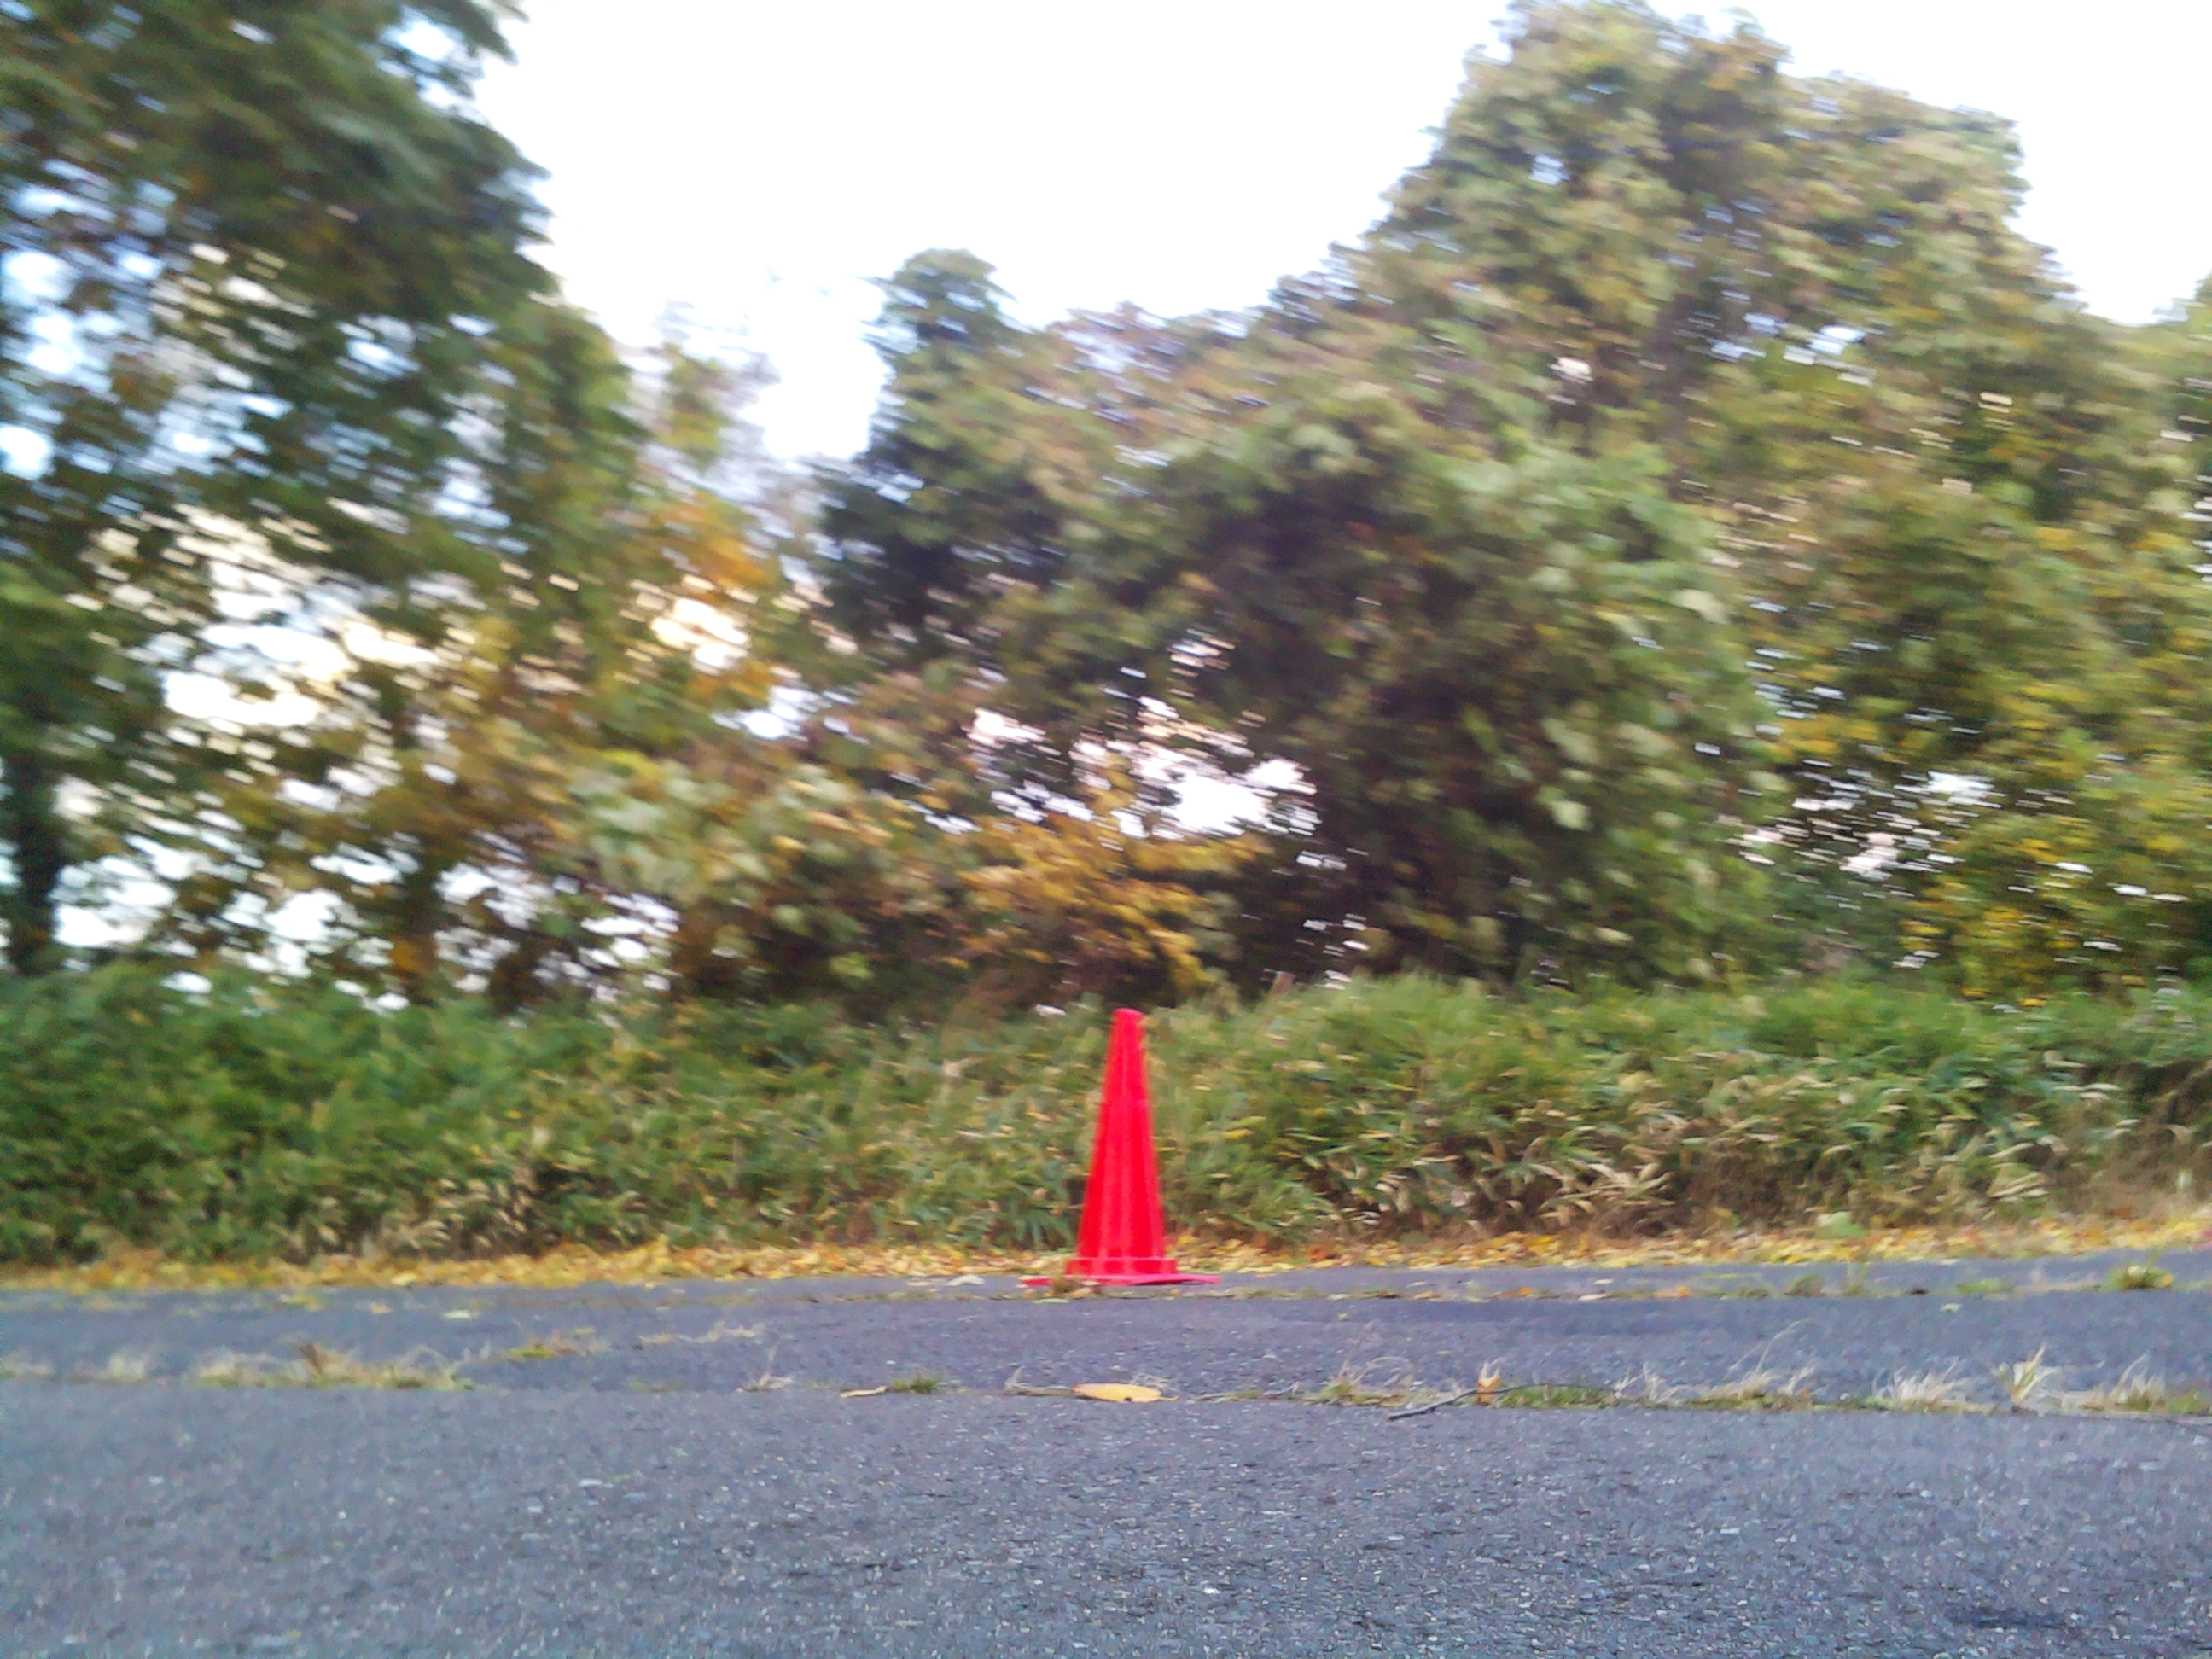
\includegraphics[width=0.4\linewidth]{../public_dataset/testdata.png}
    \caption{サンプルで用いる画像.}
    \label{fig:sample1}
\end{figure}

\section{画像処理について}
\subsection{色空間}
カラーコーン検出において,まず重要になるのが色の取り扱いである.
一般的に,画像はRGBで表現されるのが一般的であるのは周知の事実である.
色をRGBで指定することを\textbf{RGB空間}と呼ぶ.

各色の強度を0から255までの256段階 (8ビット) で表現することが多いが,
この場合,\texttt{(0, 0, 0)}が黒,\texttt{(255, 255, 255)}が白,\texttt{(255, 0, 0)}が赤,\texttt{(0, 255, 0)}が緑,\texttt{(0, 0, 255)}が青を表す.
もしくは,16進数を用いて\texttt{0x000000},\texttt{0x00FF00}のように表現することも多い.
また,さらにアルファチャンネルという透明度を表す成分を加えたRGBAで表現されることもある.
この場合,\texttt{0x00000000}が完全に透明な黒,\texttt{0xFFFFFFFF}が不透明な白を表す.

画像の処理で頻繁に用いられるOpenCVというライブラリにおいても,画像は基本この三原色で表現される.
ただし,\textbf{OpenCVでは画像はBGRの順番で表現される} ので注意が必要である
\footnote{OpenCVが開発された初期のころ,BGR形式が一般的だったためらしい.
\begin{quote}
  The reason the early developers at OpenCV chose BGR color format is that back then BGR color format was popular among camera manufacturers and software providers. E.g. in Windows, when specifying color value using COLORREF they use the BGR format 0x00bbggrr.
\end{quote}
(\href{https://learnopencv.com/why-does-opencv-use-bgr-color-format/}{Why does OpenCV use BGR color format ?}より)
}.
そのため,例えばOpenCVで処理した画像をmatplotlibで表示すると色が変わって見えることがあるが,これはBGR表記に起因するものであり,そのときはRGBに変換する必要がある.

\enskip

RGB表記は色の三原色に基づくものであるが,あまり直観的ではない.
画像処理をする上では,色相 (Hue),彩度 (Saturation),明度 (Value) の3つの成分で色を表現する\textbf{HSV空間}がよく用いられる.
ペイントエディタなどでも直観的に色を選択できるように,\cref{fig:hsv_color_wheel}のようなHSVの色相環が用いられることが多い.
\begin{figure}[H]
    \centering
    \includegraphics[width=0.3\linewidth]{figs/HSV_space.png}
    \caption{HSV色空間のイメージ図.(出典: \url{https://commons.wikimedia.org/wiki/File:Hsv_sample.png})}
    \label{fig:hsv_color_wheel}
\end{figure}

実用上でも,その場の明るさによって明度が変化することはあるが,色相は比較的変化しづらいため,色相を用いた画像認識が有用である.
なお,OpenCVでは\textbf{色相のみ範囲が0から179までの180段階で表現される}ことに注意が必要である
\footnote{参考:\url{https://docs.opencv.org/4.x/df/d9d/tutorial_py_colorspaces.html}.ソフトウェアによって異なり,0から359までの範囲で表現されることもある.}.


\subsection{色の演算}
ここについては,本番には不要であるが,画像処理の解析を行う上で知っておくと便利な演算について説明する.
読み飛ばしても差し支えない.

簡単のために,各ピクセルごとに黒 (0) か 白 (1) の2値で表現される画像を考える.
このような画像を\textbf{二値画像}と呼び,このような画像を作成することを\textbf{二値化}と呼ぶ.
このような二値画像に対しては,AND,OR,NOTなどの論理演算を行うことができる.
\begin{figure}[H]
  \centering
  \begin{minipage}
    {0.3\linewidth}
    \centering
    \includegraphics[width=\linewidth]{figs/AND.png}
    \subcaption{AND演算.}
  \end{minipage}
  \begin{minipage}
    {0.3\linewidth}
    \centering
    \includegraphics[width=\linewidth]{figs/OR.png}
    \subcaption{OR演算.}
  \end{minipage}
  \caption{AND演算とOR演算 (出典: \url{https://commons.wikimedia.org/wiki/File:Venn0001.svg}, \url{https://commons.wikimedia.org/wiki/File:Venn0111.svg}).}
  \label{fig:binary_image_operation}
\end{figure}

例えば,必要な領域を1,それ以外を0とした二値画像を用意する(このような画像を\textbf{マスク画像}と呼ぶ).
このマスク画像と元の画像に対してAND演算を行うことで,必要な領域だけを抽出することができる.
また,マスク画像を複数用意し,OR演算を行うことで,複数の領域をまとめて抽出することもできる.
本番で用いることは少ないが,処理の結果どこを検出したのかを可視化して解析する際には非常に有用である.

\subsection{モルフォロジー処理}
画像処理において,ノイズ除去や穴埋めなどの目的で\textbf{モルフォロジー処理}が用いられることがある.
例えば先の述べたようなマスク画像を作成する際,画像自体のノイズや影などの影響で,検出したい領域が途切れ途切れになってしまうことがある.
このような場合に,モルフォロジー処理を用いることで,検出したい領域を滑らかにしたり,穴埋めしたりすることができる.

モルフォロジー処理は,膨張 (Dilation) と収縮 (Erosion) の2つの基本的な操作から構成される.
膨張は,画像中の白い領域を拡大し,収縮は白い領域を縮小する操作である.
膨張によって白い領域に生じた穴が埋まり,収縮によって膨張によって拡大した領域が元の大きさに戻る.
これらの操作を組み合わせることで,ノイズ除去や穴埋めなどの効果を得ることができる.
ただし,カラーコーン検出においては膨張処理のみを行うことで不確実性を減らしている.

OpenCVでは,\texttt{cv2.morphologyEx}を用いると,様々なモルフォロジー処理を簡単に実装できる.
以下にその引数についてまとめる.

\begin{tcolorbox}[title={\texttt{cv2.morphologyEx}の引数 (必須部分のみ)\footnotemark}]
\setlength{\baselineskip}{12pt}
\begin{center}
  \texttt{cv2.morphologyEx(src, op, kernel)}
\end{center}
\begin{enumerate}
  \item \texttt{src}: 入力画像 (通常は二値画像)
  \item \texttt{op}: オプション
  \begin{enumerate}
    \item \texttt{cv2.MORPH\_DILATE}: 膨張処理 (Dilation)
    \item \texttt{cv2.MORPH\_ERODE}: 収縮処理 (Erosion)
    \item \texttt{cv2.MORPH\_OPEN}: 収縮処理 $\rightarrow$ 膨張処理 (Opening)
    \item \texttt{cv2.MORPH\_CLOSE}: 膨張処理 $\rightarrow$ 収縮処理 (Closing)
    \item \texttt{cv2.MORPH\_GRADIENT}: 勾配処理 (Gradient)
  \end{enumerate}
  \item \texttt{kernel}: カーネル (後述)
\end{enumerate}
\end{tcolorbox}
\footnotetext{参考: \url{https://docs.opencv.org/4.x/d9/d61/tutorial_py_morphological_ops.html}.}



さて,モルフォロジー処理において重要になるのが\textbf{カーネル}である.
カーネルとは,モルフォロジー処理において用いられる小さな領域であり,画像の各ピクセルに対して適用される.

例えば$5 \times 5$の大きさの正方形のカーネルを考えよう.
このカーネルを画像の各ピクセルに対して適用することで,そのピクセルの周囲$5 \times 5$の領域に対して処理が行なわれる.
例えば膨張処理の場合は,周囲$5 \times 5$の領域に白いピクセルが1つでもあれば,その中心のピクセルを白にする.
逆に収縮処理の場合は,周囲$5 \times 5$の領域が全て白でなければ,その中心のピクセルを黒にする
\footnote{一般にこのようなカーネルを用いた演算は\textbf{畳み込み演算}と呼ばれる.カーネル内での最小値が0であれば収縮,最大値が1であれば膨張となる.
また,畳み込み演算では周辺部分でカーネルを用いてどのように畳み込むかが重要となり,省略したが\texttt{cv2.morphologyEx}の引数でも指定できる.
しかしながら,カラーコーン検出ではそこまで重要でないため省略する.
}.

カーネルの形状は矩形以外にもとることができ,OpenCVでは矩形の他に十字型や楕円,菱形などを指定することもできる.
OpenCVではカーネルは以下に紹介する\texttt{cv2.getStructuringElement}で生成できる.
\begin{tcolorbox}[title={\texttt{cv2.getStructuringElement}の引数}]
\setlength{\baselineskip}{12pt}
\begin{center}
  \texttt{cv2.getStructuringElement(shape, ksize)}
\end{center}
\begin{enumerate}
  \item \texttt{shape}: カーネルの形状
  \begin{enumerate}
    \item \texttt{cv2.MORPH\_RECT}: 矩形
    \item \texttt{cv2.MORPH\_ELLIPSE}: 楕円
    \item \texttt{cv2.MORPH\_CROSS}: 十字型
    \item \texttt{cv2.MORPH\_DIAMOND}: 菱形
  \end{enumerate}
  \item \texttt{ksize}: カーネルの大きさ (タプルで指定.e.g., \texttt{(5, 5)})
  \end{enumerate}
\end{tcolorbox}





\section{色相を用いる手法}
色相を用いる手法は,カラーコーンの色相の範囲をあらかじめ決めておき,
その範囲内にあるピクセルをカラーコーンとして検出することで実現される.
非常に実装が容易であり,計算の負荷がとても低いため,堅実に動作する手法である.

ソースコードは以下の\cref{lst:hue_based_method}のようになる.
\begin{lstlisting}[caption={色相を用いる手法のサンプルコード (codes/hue.py)},label={lst:hue_based_method}]
import cv2
import numpy as np
import graph

if __name__ == "__main__":
    # Load an image from file
    image = cv2.imread("../public_dataset/testdata.png")

    # Convert the image from BGR to HSV color space
    hsv_image = cv2.cvtColor(image, cv2.COLOR_BGR2HSV)

    # Define the range for a specific hue (e.g., red color)
    lower_hue = 150
    upper_hue = 180

    # Create a mask using the defined hue range
    mask = cv2.inRange(hsv_image, (lower_hue, 100, 0), (upper_hue, 255, 255))

    # Apply the mask to the original image
    result = cv2.bitwise_and(image, image, mask=mask)

    # Display the original and resulting images
    graph.plot_result(
        image, mask, result, title1="Original", title2="Mask", title3="Result"
    )
\end{lstlisting}

コードの概略は非常にシンプルであり,特定の色相 (ここでは150から180) の範囲を定義し,その範囲にあるピクセルをマスクとして抽出している.
また,空などを誤検知するのを防ぐために,彩度についても制限を加えている.
なお,ここでは色相150 - 180をカラーコーンの色として定義しているが,例えばこれに加えて色相0 - 10を加えるならば複数のマスクを定義してOR演算を行えばよい.

画像処理による結果を以下の\cref{fig:hue_based_result}に示す.
\begin{figure}[H]
    \centering
    \includegraphics[width=\linewidth]{figs/hue_detection.pdf}
    \caption{色相を用いる手法の結果.左から元画像,マスク画像,検出結果.}
    \label{fig:hue_based_result}
\end{figure}


\section{逆投影法を用いる手法}
前章の色相を用いる手法は非常にシンプルであるが,色相を適切に指定する必要がある.
そこで,もう少し柔軟に色を検出できる手法として\textbf{逆投影法 (Back Projection)}を用いる手法がある.




\end{document}